%% Copernicus Publications Manuscript Preparation Template for LaTeX Submissions
%% ---------------------------------
%% This template should be used for copernicus.cls
%% The class file and some style files are bundled in the Copernicus Latex Package, which can be downloaded from the different journal webpages.
%% For further assistance please contact Copernicus Publications at: production@copernicus.org
%% https://publications.copernicus.org/for_authors/manuscript_preparation.html

%% copernicus_rticles_template (flag for rticles template detection - do not remove!)

%% Please use the following documentclass and journal abbreviations for discussion papers and final revised papers.

%% 2-column papers and discussion papers
\documentclass[, manuscript]{copernicus}



%% Journal abbreviations (please use the same for discussion papers and final revised papers)


% Advances in Geosciences (adgeo)
% Advances in Radio Science (ars)
% Advances in Science and Research (asr)
% Advances in Statistical Climatology, Meteorology and Oceanography (ascmo)
% Annales Geophysicae (angeo)
% Archives Animal Breeding (aab)
% ASTRA Proceedings (ap)
% Atmospheric Chemistry and Physics (acp)
% Atmospheric Measurement Techniques (amt)
% Biogeosciences (bg)
% Climate of the Past (cp)
% DEUQUA Special Publications (deuquasp)
% Drinking Water Engineering and Science (dwes)
% Earth Surface Dynamics (esurf)
% Earth System Dynamics (esd)
% Earth System Science Data (essd)
% E&G Quaternary Science Journal (egqsj)
% European Journal of Mineralogy (ejm)
% Fossil Record (fr)
% Geochronology (gchron)
% Geographica Helvetica (gh)
% Geoscience Communication (gc)
% Geoscientific Instrumentation, Methods and Data Systems (gi)
% Geoscientific Model Development (gmd)
% History of Geo- and Space Sciences (hgss)
% Hydrology and Earth System Sciences (hess)
% Journal of Bone and Joint Infection (jbji)
% Journal of Micropalaeontology (jm)
% Journal of Sensors and Sensor Systems (jsss)
% Magnetic Resonance (mr)
% Mechanical Sciences (ms)
% Natural Hazards and Earth System Sciences (nhess)
% Nonlinear Processes in Geophysics (npg)
% Ocean Science (os)
% Polarforschung - Journal of the German Society for Polar Research (polf)
% Primate Biology (pb)
% Proceedings of the International Association of Hydrological Sciences (piahs)
% Scientific Drilling (sd)
% SOIL (soil)
% Solid Earth (se)
% The Cryosphere (tc)
% Weather and Climate Dynamics (wcd)
% Web Ecology (we)
% Wind Energy Science (wes)


%% \usepackage commands included in the copernicus.cls:
%\usepackage[german, english]{babel}
%\usepackage{tabularx}
%\usepackage{cancel}
%\usepackage{multirow}
%\usepackage{supertabular}
%\usepackage{algorithmic}
%\usepackage{algorithm}
%\usepackage{amsthm}
%\usepackage{float}
%\usepackage{subfig}
%\usepackage{rotating}

% Pandoc citation processing

% The "Technical instructions for LaTex" by Copernicus require _not_ to insert any additional packages.
%%\usepackage{booktabs}
\usepackage{longtable}
\usepackage{array}
\usepackage{multirow}
\usepackage{wrapfig}
\usepackage{float}
\usepackage{colortbl}
\usepackage{pdflscape}
\usepackage{tabu}
\usepackage{threeparttable}
\usepackage{threeparttablex}
\usepackage[normalem]{ulem}
\usepackage{makecell}
\usepackage{xcolor}
%
\usepackage{algorithmic}
\usepackage{algorithm}


\begin{document}

\title{Informing IPCC accounting of forest carbon using the global
forest carbon database (ForC v4.0)}


\Author[1]{Madison}{Williams}
\Author[1]{Valentine}{Herrmann}
\Author[1,2]{Rebecca}{Banbury Morgan}
\Author[3]{Ben}{Bond-Lamberty}
\Author[4]{Susan}{Cook-Patton}
\Author[5]{Sandro}{Federici}
\Author[6]{Helene}{Muller-Landau}
\Author[7]{Camille}{Piponiot}
\Author[1]{Teagan}{Rogers}
\Author[5]{Valentyna}{Slivinska}
\Author[1,6 *]{Kristina J.}{Anderson-Teixeira}


\affil[1]{Center for Conservatiton Ecology, Smithsonian Conservation
Biology Institute, Front Royal, VA, United States}
\affil[2]{School of Geography, University of Leeds, Leeds, UK}
\affil[3]{Joint Global Change Research Institute, Pacific Northwest
National Laboratory, College Park, MD, United States}
\affil[4]{The Nature Conservancy; Arlington VA 22203, USA}
\affil[5]{IPCC Task Force on National Greenhouse Gas Inventories
Technical Support Unit, Institute for Global Environmental Strategies,
Hayama, Japan}
\affil[6]{Forest Global Earth Observatory, Smithsonian Tropical Research
Institute, Panama, Republic of Panama}
\affil[7]{CIRAD, Montpellier, France}

\runningtitle{IPCC forest C accounting with ForC}

\runningauthor{Williams et al.}


\correspondence{Kristina J.\ Anderson-Teixeira\ (teixeirak@si.edu)}



\received{}
\pubdiscuss{} %% only important for two-stage journals
\revised{}
\accepted{}
\published{}

%% These dates will be inserted by Copernicus Publications during the typesetting process.


\firstpage{1}

\maketitle


\begin{abstract}
The abstract goes here. It can also be on \emph{multiple lines}.
\end{abstract}


\copyrightstatement{The author's copyright for this publication is
transferred to institution/company.}


\textbf{Important}: Always double-check with the official manuscript
preparation guidelines at
\url{https://publications.copernicus.org/for_authors/manuscript_preparation.html},
especially the sections ``Technical instructions for LaTeX'' and
``Manuscript composition''. Please contact Daniel Nüst,
\texttt{daniel.nuest@uni-muenster.de}, with any problems.

\introduction[Introduction]

\textbf{As we seek to mitigate climate change
\citep{unfccc_adoption_2015}, forests are critical.} \emph{(See intros
to other papers for relevant refs)} Under Paris Agreement,
\textbf{\#\#}\% of Nationally Determined Contributions relate to forests
\citep{grassi_key_2017}.

\textbf{The International Panel on Climate Change (IPCC) provides
guidance for national greenhouse gas (GHG) inventories for reporting to
the United Nations Framework Convention on Climate Change \citep[UNFCCC,
(REFS for older guidelines),][]{ipcc_2019_2019}.} Under this guidance,
GHG inventories include all managed land, including most of the world's
forest land \citep{ogle_delineating_2018}. The IPCC inventory guidelines
include specific instructions for accounting for forest land \ldots{}
\citep{ipcc_agriculture_2006, ipcc_2019_2019a}. This guidance has
improved as more of the relevant underlying data has become available
\citep{requenasuarez_estimating_2019}, but there remains room for
continuous improvement as the science advances. For example,
\citet{cook-patton_mapping_2020} \emph{(summarize IPCC comparison
results)}. \emph{Moreover, it is useful for those compiling national
greenhouse gas inventories to have access to locally-specific
information, when available.} To improve the data accessible for C
accounting, the IPCC created the Emission Factor Database (EFDB;
https://www.ipcc-nggip.iges.or.jp/EFDB/main.php), which is intended as a
recognized library of emission factors and other parameters that can be
used for estimating greenhouse gas emissions and removals.

\textbf{The Global Forest Carbon Database, ForC, is the largest
collection of published estimates of forest carbon stocks, increments,
and annual fluxes
\citep{anderson-teixeira_forc_2018, anderson-teixeira_carbon_2021}.}
\emph{(add stats/ details)} As such, ForC is positioned to improve
forest C accounting through the transfer of data to EFDB. The purpose of
this publication is to document that process and provide recommendations
for future improvements.

\textbf{Here, we} (1) review definitions of relevant carbon stocks and
increments (2) describe mapping of ForC to IPCC's EFDB, (3) describe
updates to ForC (ForC v4.0), (4) summarize the data in ForC that's
relevant to EFDB, identifying gaps, and (5) provide recommendations for
improving data collection, analysis, database, and accounting.

\section{Defining carbon stocks and incremenets}

For quantifying forest role in global C cycle, we ultimately care about:
(1) C stocks -- stores of C that would be vulnerable to release to the
atmosphere upon land use change (2) C increments -- changes in those C
stocks.

\subsection{Carbon stocks}

Forest ecosystem C stocks may be parsed into pools in various ways. IPCC
parses into biomass (aboveground and belowground), dead organic matter
(dead wood and litter), and soil organic matter
(Table~@ref(table\_variables)). Quantifying these requires a one-time
measurement.

\subsubsection{Biomass}

Biomass includes living vegetation, above- and below-ground.

The IPCC defines aboveground biomass as ``all biomass of living
vegetation, both woody and herbaceous, above the soil including stems,
stumps, branches, bark, seeds, and foliage'' {[}{]}.

Belowground biomass is defined as ``all biomass of live roots'' {[}{]}.

\subsubsection{Dead Organic Matter}

\subsubsection{Soil Organic Matter}

\begin{table}

\caption{\label{tab:table_variables}\textbf{Variables with definitions and measurement methods.} Definitions from IPCC Table 1.1. (See Table 1.1 in IPCC guidance).}
\centering
\begin{tabu} to \linewidth {>{\raggedright}X>{\raggedright}X>{\raggedright}X>{\raggedright}X}
\hline
\textbf{pool} & \textbf{definition} & \textbf{major sources of estimate variation} & \textbf{IPCC guidance}\\
\hline
aboveground biomass & all biomass of living vegetation, both woody and herbaceous, above the soil & allometry, min dbh & acceptable to exclude understory\\
\hline
belowground biomass & all biomass of live roots & allometry, min dbh, assumed ratio of belowground to aboveground biomass (IPCC table 4.4) & fine roots may be excluded when they cannot be distinguished empirically from soil organic matter or litter\\
\hline
dead wood & all non-living woody biomass not contained in the litter, either standing, lying on the ground, or in the soil & min dbh,  ... & default min dbh = 10cm, but may be chosen by country\\
\hline
litter & all non-living biomass with a size greater than the limit for soil organic matter  and less than the minimum diameter chosen for dead wood, lying dead, in various states of decomposition above or within the mineral or organic soil & min dbh for dead wood , .. & \\
\hline
soil organic matter & organic carbon in mineral soils to a specified depth & sampling depth & default sampling depth = 30cm, but may be chosen by country\\
\hline
\end{tabu}
\end{table}

\subsection{Carbon increments}

C increments are defined as the change over time, in annual increments,
in each C pool. These may be estimated as the difference between C
stocks at two time points, or as the difference between inputs and
outputs to the pool (i.e., fluxes). Quantifying these requires at least
two measurements.

Fluxes are the inputs and outputs to each pool.

\begin{figure}
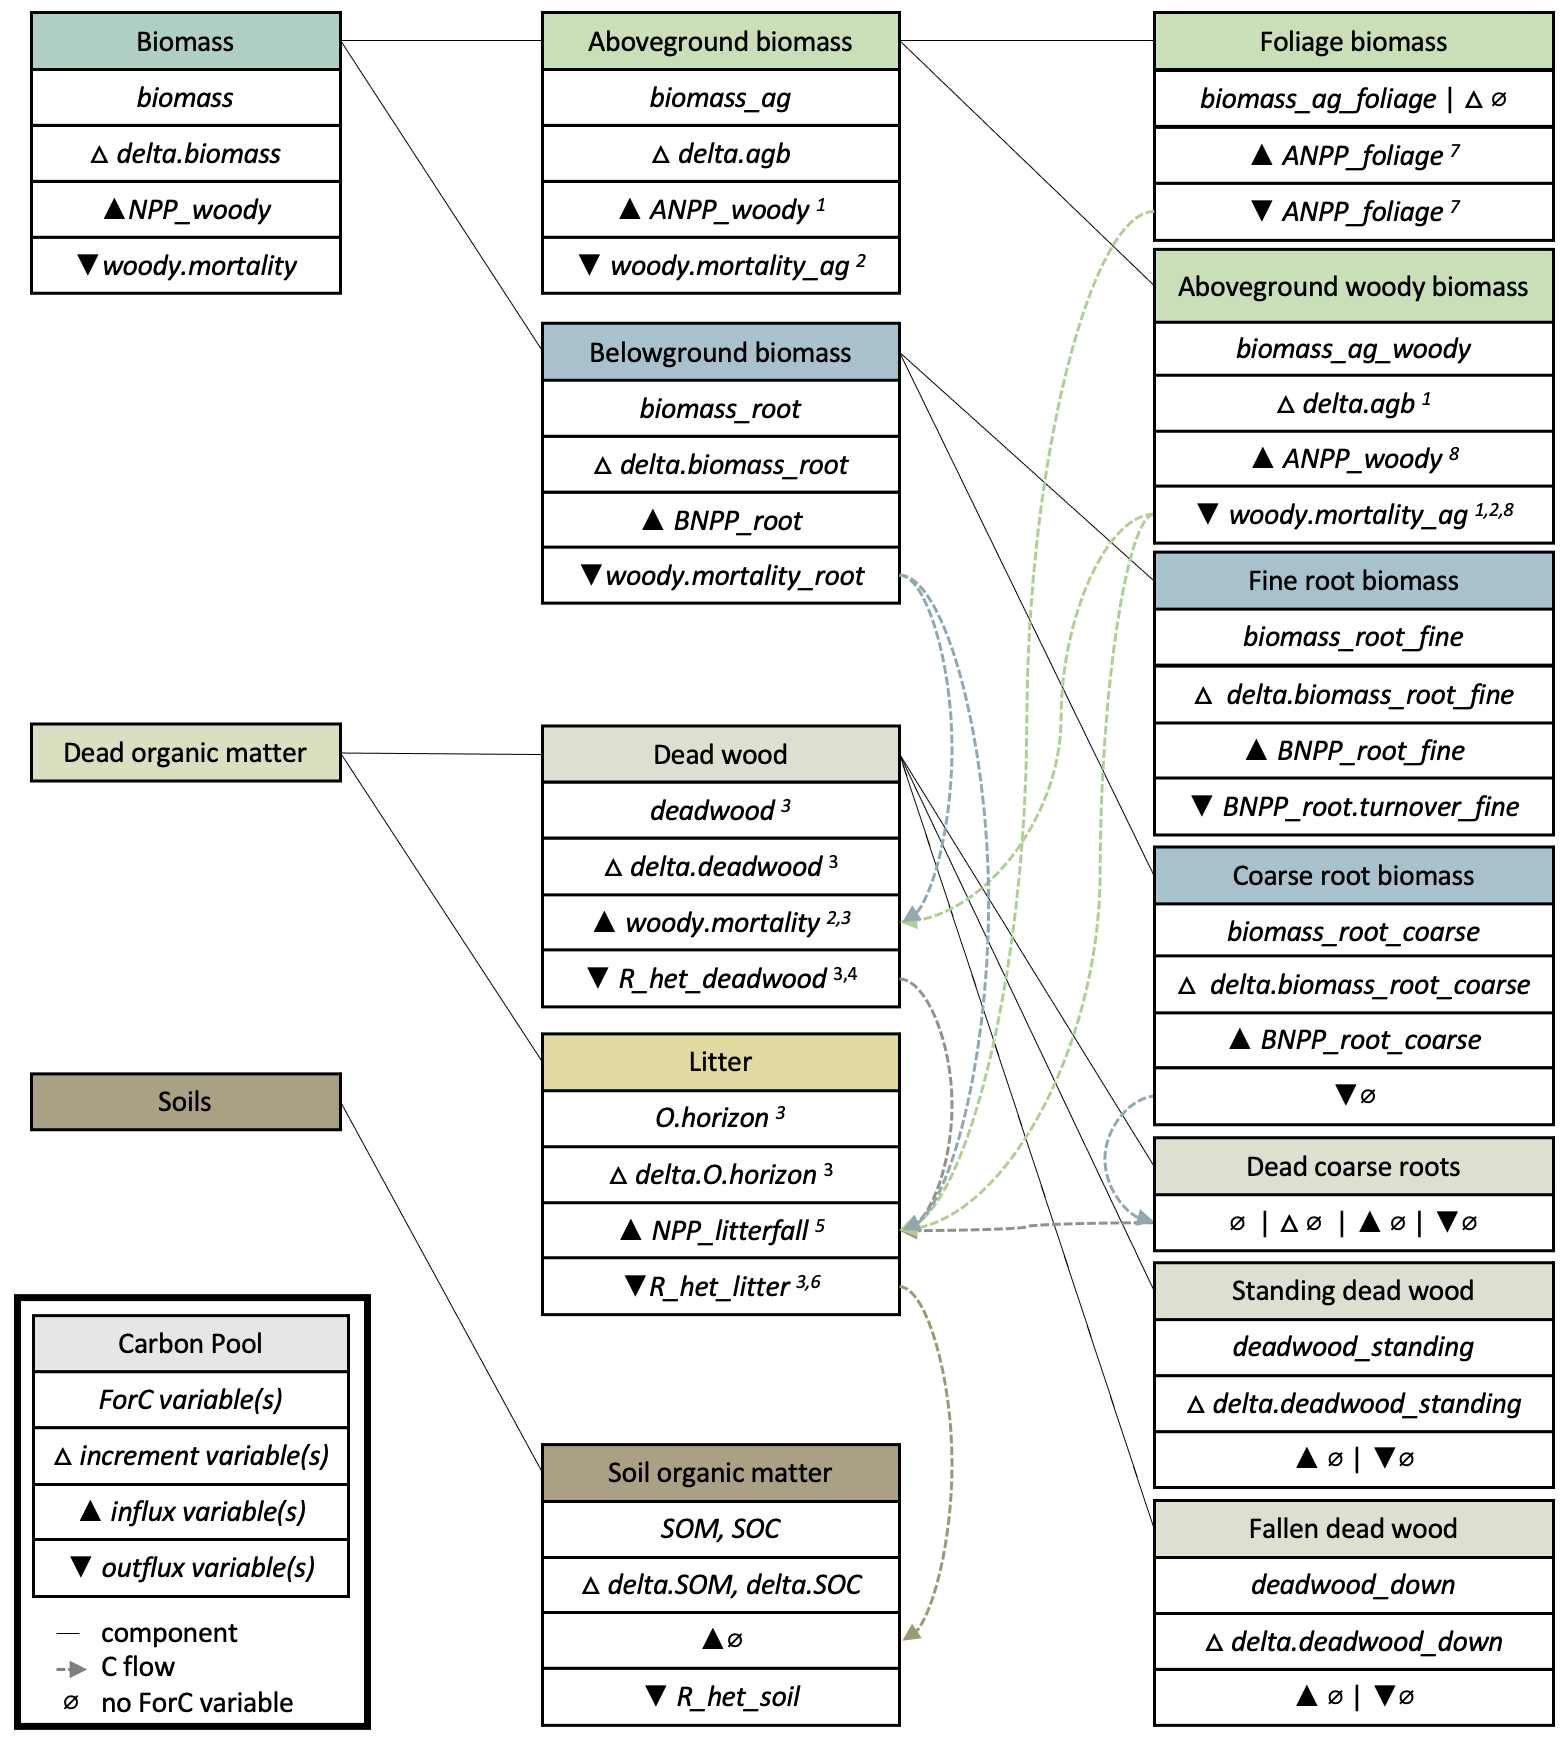
\includegraphics[width=15cm]{figures_tables/C_variable_mapping} \caption{\textbf{Schematic illustrating the carbon pools quantified under IPCC accounting; ForC variables corresponding to the stock, increment, influx and outflux; and relationships among them.} In many cases, the match of ForC variables to IPCC criteria depends upon measurement protocols (e.g., minimum DBH). Additional caveats are as follows: 1- assumes minimal non-respiratory C fluxes,... (Chapin et al. 2006); 2- assumes that change in foliage biomass is negligible (see note 7); 3- incomplete: excludes large branch fall; also, under IPCC definitions, outflux from aboveground biomass should include all sizes, influx to deadwood should include only above the minimum diameter chosen for dead wood; 4- incomplete: excludes belowground components;  5-incomplete: excludes breakage into pieces less than dead wood threshold size; 6-incomplete: excludes woody mortality of stems <10 cm DBH, decomposition of dead wood (aboveground and coarse roots) into sizes classified as litter; 7-foliage production is generally measured by collecting leaf-fall, a method that assumes that the influx = outflux (foliage biomass is roughly constant year-to-year).}\label{fig:unnamed-chunk-1}
\end{figure}

\section{Mapping ForC to EFDB}

\subsection{Carbon cycle variables}

Mapping is shown in Fig. 1

Define relationship among NEE, NEP, and delta.C., especially noting role
of harvest \citep{chapin_reconciling_2006}.

\subsection{Land use categories}

Documented at
https://github.com/forc-db/IPCC-EFDB-integration/blob/main/doc/ForC-EFDB\_mapping/defining\_land\_subcategory.md,
https://github.com/forc-db/IPCC-EFDB-integration/blob/main/doc/ForC-EFDB\_mapping/IPCC\_LandUse\_mapping.csv,
and in
\href{https://github.com/forc-db/IPCC_database_integration/issues/8}{issue
\#8}.

The UNFCCC requires GHG reporting for all managed lands in a country,
where management is defined as ``human interventions and practices have
been applied to perform production, ecological or social functions''
{[}\emph{IPCC 2006 full report REF}{]}. This definition is applied
differently across countries, and is not clearly defined by the majority
of governments \citep{ogle_delineating_2018}. Given this, and because
the IPCC definition of management does not necessarily match that which
would be reported in scientific publications and hence in ForC, we do
not transfer any classification of land management status from ForC to
the EFDB, but do provide auxiliary info that may be useful in making
this determination (e.g., geographical location).

\section{Updates to ForC (ForC v4.0)}

To support export of data to EFDB, and to improve the overall quality of
the ForC database, we added ten increment variables, implemented some
modest restructuring, resolved duplicate records, and conducted quality
control. This section describes changes relative to ForC v2.0
\citep{anderson-teixeira_forc_2018}.

\subsection{Increment variables}

We added ten increment variables to the set of named and defined
variables (or 20, counting \_OM and \_C versions), which previously
included only one (aboveground biomass increment, \emph{delta.agb}).
\emph{(https://github.com/forc-db/IPCC-EFDB-integration/issues/6)} These
are directly related to C stocks as previously defined in ForC, with
``\emph{delta.}'' added in front of the variable name.

Although these variables currently lack records, the structure exists
such that records can be populated over time.

\subsection{ForC restructuring}

\begin{table}

\caption{\label{tab:table_ForCchanges}\textbf{Table of changes to ForC fields.}}
\centering
\begin{tabu} to \linewidth {>{\raggedright}X>{\raggedright}X>{\raggedright}X>{\raggedright}X>{\raggedright}X}
\hline
\textbf{Table} & \textbf{Column} & \textbf{Description} & \textbf{Changes} & \textbf{Motivation}\\
\hline
Sites & coordinates.precision & Precision of geographic coordinates, as reported by source or estimated from maps. & field added & allow identification of records with poor coordinate precision\\
\hline
Measuremennts & data.location.within.source & Location of data within the source listed in citation.ID. & field added & facilitate review, ensure traceability\\
\hline
 & sd, se, lower95\%CI, upper 95\%CI & Standard deviation, standard error, and lower and upper 95 percent confidence intvervals, respectively. & replaces `stat` and `stat.name` & cleaner format; ability to handle assymetrical 95 percent confidence intervals\\
\hline
 & mean.in.original.units, original.units & mean value and units presented in original publication & fields added & provide IPCC with original units, reduce errors/improve reproducibility\\
\hline
 & C.conversion.factor & Assumed/ measured C content of organic matter used to convert organic matter to C. & field added & track units conversion, allow back-calculation of OM if conversion factor deemed inappropriate\\
\hline
PFT & description & Definition of the pftcode at the community level. Differs from individual level in that properly describes mixed plant functional types. & field added & \\
\hline
 & description.individual & Definition of the pftcode at the individual plant level. & field name change (previously `description`) & \\
\hline
Citations & (several fields) &  &  & \\
\hline
\end{tabu}
\end{table}

\subsection{Quality control measures}

Prior to releasing ForC v4.0, we executed several quality control
measures. First, to improve information on geographic coordinates, we
flagged and reviewed records with suspected low precision \emph{(Issue
\#29){[}https://github.com/forc-db/ForC/issues/229{]}}. Second, to
identify erroneous climate data\ldots{} \emph{(Issue
\#212){[}https://github.com/forc-db/ForC/issues/212{]}}.

\subsection{Resolving duplicates}

\section{Results}

\textbf{figure: map of relevant ForC data with underlying FAO ecozones}

\textbf{(summarize the data in ForC that's relevant to EFDB, identifying
gaps)}

dead wood and litter comparisons will be particularly interesting, as
IPCC values are based on just a handful of references for each climate
zone (table 2.2 in 2019 guidelines)

\section{Recommendations}

\subsection{Data collection and analysis needs}

\textbf{(Paragraph highlighting important gaps in variables / regions)}

Several variables of value to IPCC, including standing dead wood, woody
mortality, delta.agb, are not calculated and presented as frequently as
are AGB and ANPP\_woody, even though they can readily be derived from
the same census data. We recommend that researchers calculate and report
these, as specified below. Furthermore, there is an opportunity to fill
data gaps by calculating these from existing census data. For example,
the core census protocol of the Forest Global Earth Observatory
{[}ForestGEO; REFS{]} collects the data required to calculate standing
dead wood, woody mortality, and delta.agb, but these have not been
calculated and reported for all sites for which the appropriate number
of censuses are available (n=1 for standing dead wood, n=2 for woody
mortality and delta.agb) {[}but see REFS{]}.

A universal challenge in estimating biomass (living or dead) from forest
census data is applying appropriate allometries to convert DBH
measurements to biomass. \emph{(Camille/Helene can write this paragraph
easily.)}

\subsection{Data reporting needs}

We recommend that, unless they have some specific reason to do
otherwise, researchers calculate and report the values according to IPCC
standards:

\begin{itemize}
\item
  adopt common standards for variables like min diameter of deadwood,
  select soil sampling increments to include a cutoff at 30.
\item
  report 95\% CIs, SE, or STD and n
\item
  report C variables in article text, table, or SI table. EFDB cannot
  accept data digitized from figures
\end{itemize}

For data synthesis projects, compilation can only be useful to the EFDB
if they include all the required, along with transparent description on
the methodology applied to derive emission factors (or have a brief
description and a reference to the original source) and the original
emission factor values are present (not modified/rounded).

\textbf{Contributing data to ForC and/or EFDB directly will ensure its
broader impact.} The latter is more efficient for getting data to EFDB,
but does not get the data into ForC, where it can be more broadly
useful--for example, being used for basic science
\citep[e.g.,][]{banburymorgan_global_2021, anderson-teixeira_carbon_2021}
or model benchmarking \citep{fer_ecosystem_2021}.

\subsection{Database needs}

There are plenty of relevant, published data that are not included in
ForC. Systematic review of the literature could vastly improve data
coverage. \emph{(There are some efforts underway, including a few that
Susan can specify.)}

\subsection{IPCC}

An important challenge is that forests are changing rapidly, and data
collected a decaade ago may no longer be relevant, particularly in the
cases of C increments and fluxes.

Remote sensing biomass estimates include standing dead wood
\citep{duncanson_aboveground_2021}.

\conclusions[Conclusions]

The conclusion goes here. You can modify the section name with
\texttt{\textbackslash{}conclusions{[}modified\ heading\ if\ necessary{]}}.



\codedataavailability{use this to add a statement when having data sets
and software code
available} %% use this section when having data sets and software code available



%%%%%%%%%%%%%%%%%%%%%%%%%%%%%%%%%%%%%%%%%%
%% optional

%%%%%%%%%%%%%%%%%%%%%%%%%%%%%%%%%%%%%%%%%%

%%%%%%%%%%%%%%%%%%%%%%%%%%%%%%%%%%%%%%%%%%
\authorcontribution{(fill this in)} %% optional section

%%%%%%%%%%%%%%%%%%%%%%%%%%%%%%%%%%%%%%%%%%
\competinginterests{The authors declare no competing
interests.} %% this section is mandatory even if you declare that no competing interests are present

%%%%%%%%%%%%%%%%%%%%%%%%%%%%%%%%%%%%%%%%%%

%%%%%%%%%%%%%%%%%%%%%%%%%%%%%%%%%%%%%%%%%%
\begin{acknowledgements}
Thank you to all researchers who collected and published the data
contained in ForC, and to all research assistants and collaborators who
have helped to build the database. Funding for this study was provided
by The Nature Conservancy, the Institute for Global Environmental
Strategies, WLS(?)
\end{acknowledgements}

%% REFERENCES
%% DN: pre-configured to BibTeX for rticles

%% The reference list is compiled as follows:
%%
%% \begin{thebibliography}{}
%%
%% \bibitem[AUTHOR(YEAR)]{LABEL1}
%% REFERENCE 1
%%
%% \bibitem[AUTHOR(YEAR)]{LABEL2}
%% REFERENCE 2
%%
%% \end{thebibliography}

%% Since the Copernicus LaTeX package includes the BibTeX style file copernicus.bst,
%% authors experienced with BibTeX only have to include the following two lines:
%%
\bibliographystyle{copernicus}
\bibliography{references.bib}
%%
%% URLs and DOIs can be entered in your BibTeX file as:
%%
%% URL = {http://www.xyz.org/~jones/idx_g.htm}
%% DOI = {10.5194/xyz}


%% LITERATURE CITATIONS
%%
%% command                        & example result
%% \citet{jones90}|               & Jones et al. (1990)
%% \citep{jones90}|               & (Jones et al., 1990)
%% \citep{jones90,jones93}|       & (Jones et al., 1990, 1993)
%% \citep[p.~32]{jones90}|        & (Jones et al., 1990, p.~32)
%% \citep[e.g.,][]{jones90}|      & (e.g., Jones et al., 1990)
%% \citep[e.g.,][p.~32]{jones90}| & (e.g., Jones et al., 1990, p.~32)
%% \citeauthor{jones90}|          & Jones et al.
%% \citeyear{jones90}|            & 1990

\end{document}
